\chapter{Appendix}
\section{List of Boosters}\label{boosters}
In the following table there are all the various boosters with their description, effect, usage condition and how they look like in the game. Each row represents one booster.
\begin{table}[H]
    \caption{Full list and description of boosters}
    \centering
    \tiny
    
    \begin{tabular}{
  >{\raggedright\arraybackslash}m{.1\linewidth} % col width
  >{\centering\arraybackslash}m{.05\linewidth} % col width
  >{\arraybackslash}m{.1\linewidth} % col width
  >{\raggedright\arraybackslash}m{.1\linewidth} % col width
  >{\arraybackslash}m{.35\linewidth} % col width
}
    \toprule
    \textbf{Name} & \textbf{Image} & \textbf{Type} & \textbf{Levels} & \textbf{Effect} \\
    \midrule
    Lollipop Hammer & 
    
\includegraphics[width=0.04\textwidth]{masters-thesis-master/masters-thesis/contents/a_appendix/booster_images/Booster_lollipop_hammer.png} &
    In-level &
    All levels &
    Smash a candy (or a blockers) except chocolate spawner, ingredients, toffee tornado or sugar chest and destroy it.\\ 
    Extra Moves +5 & 
    
\includegraphics[width=0.04\textwidth]{masters-thesis-master/masters-thesis/contents/a_appendix/booster_images/Booster_extra_moves_5.png} &
    In-level, consolation &
    All except timed levels &
    Adds five additional extra moves.\\ 
    Extra Moves +3 & 
    
\includegraphics[width=0.04\textwidth]{masters-thesis-master/masters-thesis/contents/a_appendix/booster_images/Booster_extra_moves_3.png} &
    Pre-level &
    All except timed levels &
    Adds three additional extra moves.\\
    Jelly Fish & 
    
\includegraphics[width=0.04\textwidth]{masters-thesis-master/masters-thesis/contents/a_appendix/booster_images/Booster_jelly_fish.png} &
    Pre-level &
    Jelly levels &
    Spawn 3 jelly fish at random on the gameboard.\\ 
    Colour Bomb & 
    
\includegraphics[width=0.04\textwidth]{masters-thesis-master/masters-thesis/contents/a_appendix/booster_images/Booster_color_bomb.png} &
    Pre-level &
    All levels &
    Start with one colour bomb on the gameboard.\\ 
    Coconut Wheel & 
    
\includegraphics[width=0.04\textwidth]{masters-thesis-master/masters-thesis/contents/a_appendix/booster_images/Booster_coconut_wheel.png} &
    Pre-level &
    Ingredients levels &
    Spawn a coconut wheel on the gameboard.\\ 
    Free Switch & 
    
\includegraphics[width=0.04\textwidth]{masters-thesis-master/masters-thesis/contents/a_appendix/booster_images/Booster_free_switch.png} &
    In-level &
    All levels &
    Allows the player to switch 2 candies even if they do not match.\\ 
    % Extra Time & 
    % 
\includegraphics[width=0.04\textwidth]{masters-thesis-master/masters-thesis/contents/a_appendix/booster_images/Booster_extra_time.png} &
    % Pre-level, consolation &
    % Timed levels &
    % Adds fifteen extra seconds on timed levels.\\ 
    Striped and Wrapped & 
    
\includegraphics[width=0.04\textwidth]{masters-thesis-master/masters-thesis/contents/a_appendix/booster_images/Booster_striped_and_wrapped.png} &
    Pre-level &
    All levels &
    Start the game with a wrapped and a striped candy on the gameboard.\\ 
    % Sweet Teeth & 
    % 
\includegraphics[width=0.04\textwidth]{masters-thesis-master/masters-thesis/contents/a_appendix/booster_images/Booster_sweet_teeth.png} &
    % In-level &
    % All levels &
    % Eats several candies, liquorice, chocolate, icing and marmalade.\\ 
    Bomb Cooler & 
    
\includegraphics[width=0.04\textwidth]{masters-thesis-master/masters-thesis/contents/a_appendix/booster_images/Booster_bomb_cooler.png} &
    In-level &
    All levels &
    Adds five extra moves to Candy Bombs. Available only if there are Candy Bombs on the gameboard.\\
    Lucky Candy & 
    
\includegraphics[width=0.04\textwidth]{masters-thesis-master/masters-thesis/contents/a_appendix/booster_images/Booster_lucky_candy.png} &
    Pre-level &
    Order levels &
    Spawn a lucky candy on the gameboard.\\ 
    % Bubblegum Troll & 
    % 
\includegraphics[width=0.04\textwidth]{masters-thesis-master/masters-thesis/contents/a_appendix/booster_images/Booster_bubblegum_troll.png} &
    % In-level &
    % Levels with chocolate spawners &
    % Removes all chocolate and stop the chocolate spawners for 5 moves.\\ 
    UFO & 
    
\includegraphics[width=0.04\textwidth]{masters-thesis-master/masters-thesis/contents/a_appendix/booster_images/Booster_UFO.png} &
    Pre-level &
    All levels &
    Spawn a UFO on the gameboard.\\ 
    Striped Brush & 
    
\includegraphics[width=0.04\textwidth]{masters-thesis-master/masters-thesis/contents/a_appendix/booster_images/Booster_Striped_Brush.png} &
    In-level &
    All levels &
    Allows the player to convert any regular candy into a striped candy and to choose the directions of the stripes.\\
    Party Popper & 
    
\includegraphics[width=0.04\textwidth]{masters-thesis-master/masters-thesis/contents/a_appendix/booster_images/Party_Popper_Booster.png} &
    In-level &
    All levels &
    Clears the gameboard and adds special candies.\\
    \bottomrule
    \end{tabular}

% After that, you can buy more boosters if you want to use them.
% You can also get free boosters in various ways. You can be awarded boosters by completing usually 10 levels in some games by King.com, and refill your lives. There is one booster that is only available when a Facebook or King.com friend sends you one, namely the +3 moves booster.
% As of November 27, 2013, players can obtain free boosters every day from the daily booster wheel.
% As of April 22, 2015, some players can obtain free boosters by collecting Sugar Drops on specially marked levels.
% When the player completes the final level in the Dreamworld for the first time, the player receives an award equivalent to the Jackpot.
% Some of the events will provide boosters as rewards upon completing the objective.
% In rare case if an event is glitched, there will be some boosters for making up.
% Owing to the rarity, almost all main walkthrough videos involve gameplay without boosters, and will give special notice if they are using boosters.


% Note1: Boosters shown in bold are available only in the web version, not on mobile.

% Note2: Boosters shown in strikeout are no longer available on any device.




    \label{tab:boosters}
\end{table}

\section{Supplement Information Regarding CNN Inputs}
In the following table there are all the input features of the \ac{CNN}. Each row represents one feature layer.
\FloatBarrier
\begin{table}[H]
    \caption{Full list of input features (1/2)}
    \centering
    \tiny
        \begin{tabular}{l l}
    \toprule
    \textbf{Layers} \\%& \textbf{Comments} \\
    \midrule
  
    REGULAR\_CANDY \\%& Encodes that the candy on that position is a regular candy\\   
    PEPPER\_CANDY \\%& Explode after a certain number of moves leading to failing the objective\\   
    MYSTERY\_CANDY \\%& Mystery candies spawn a random item when being destroyed\\   
    CHAMELEON\_CANDY \\%& A chameleon candy is a candy that changes it's color after every move\\   
    CANDY\_COLOR \\   
    CANDY\_COLOR\_RED \\   
    CANDY\_COLOR\_YELLOW \\   
    CANDY\_COLOR\_BLUE \\   
    CANDY\_COLOR\_GREEN \\   
    CANDY\_COLOR\_ORANGE \\   
    CANDY\_COLOR\_PURPLE \\   
    FISH \\   
    CANDY\_STRIPED\_LINE \\   
    CANDY\_STRIPED\_COLUMN \\   
    CANDY\_WRAPPED \\   
    LUCKY\_CANDY \\   

    VOID \\   
    EMPTY \\   
    LIGHT\_1 \\   
    LIGHT\_2 \\   
    CANDY\_CANNON \\ 
    STATIC\_BLOCKER \\ 
    FROSTING \\   
    LIQUORICE\_LOCK \\   
    FUDGE \\  
    INGREDIENT\_COLLECTOR \\   
    PORTAL \\ 
    PORTAL\_ENTER\_POINT \\   
    PORTAL\_EXIT\_POINT \\  
    PORTAL\_VISIBLE \\  
    PORTAL\_VISIBLE\_ENTER\_POINT \\ 
    PORTAL\_VISIBLE\_EXIT\_POINT \\  
    LICORICE\_SQUARE \\   
    MULTI\_FROSTING\_1 \\   
    MULTI\_FROSTING\_2 \\  
    MULTI\_FROSTING\_3 \\   
    MULTI\_FROSTING\_4 \\
    MULTI\_FROSTING\_5 \\ 
    CHOCOLATE\_SPAWNER \\   
    MARMELADE\_LOCK \\   
    DIVINE\_DROP \\   
    SUGAR\_DROP \\ 
    CANDY\_CANNON\_AMMO\_CANDY \\ 
    CANDY\_CANNON\_AMMO\_INGREDIENT \\ 
    CANDY\_CANNON\_AMMO\_LIQUORICE\_SQUARE \\ 
    CANDY\_CANNON\_AMMO\_PEPPER \\ 
    CANDY\_CANNON\_AMMO\_MULOCK\_CANDY \\ 
    CANDY\_CANNON\_AMMO\_MYSTERY\_CANDY \\ 
    CAKE\_BOMB \\   
    JELLY\_FROG \\ 
    MULOCK\_1 \\   
    MULOCK\_2 \\   
    MULOCK\_3 \\   
    MULOCK\_4 \\   
    MULOCK\_5 \\   
    

        
    \bottomrule
    \end{tabular}

    \label{tab:features_1}
\end{table}

\begin{table}[H]
    \caption{Full list of input features (2/2)}
    \centering
    \tiny
        \begin{tabular}{l}
    \toprule
    \textbf{Layers} \\%& \textbf{Explanation} \\
    \midrule
    COCONUT\_WHEEL \\   
    INGREDIENT \\   
    EXTRA\_TIME \\ 
    MULOCK\_KEY \\   
    CHOCOLATE\_FROG \\ 
    POPCORN \\   
    UFO \\   
    EVIL\_SPAWNER \\   
    FROGGER\_EXIT \\ 
    JELLY\_COLOR\_GREEN \\   
    JELLY\_COLOR\_RED \\   
    BOBBER \\ 
    CANDY\_CANNON\_AMMO\_CHAMELEON \\ 
    CANDY\_CANNON\_AMMO\_LUCKY \\ 
    CANDY\_CANNON\_AMMO\_TIME \\ 

    CONVEYOR\_BELT \\ 
    CONVEYOR\_BELT\_UP \\   
    CONVEYOR\_BELT\_RIGHT \\   
    CONVEYOR\_BELT\_DOWN \\   
    CONVEYOR\_BELT\_LEFT \\   

    CONVEYOR\_BELT\_PORTAL \\ 
    CONVEYOR\_BELT\_PORTAL\_NONE \\ 
    CONVEYOR\_BELT\_PORTAL\_RED \\   
    CONVEYOR\_BELT\_PORTAL\_BLUE \\   
    CONVEYOR\_BELT\_PORTAL\_GREEN \\   

  
    
    % **** Candy Orders ****
    % **** single ****
    ORDER\_CANDY\_COLOR\_RED \\ 
    ORDER\_CANDY\_COLOR\_BLUE \\ 
    ORDER\_CANDY\_COLOR\_YELLOW \\ 
    ORDER\_CANDY\_COLOR\_ORANGE \\ 
    ORDER\_CANDY\_COLOR\_PURPLE \\ 
    ORDER\_CANDY\_COLOR\_GREEN \\ 
    ORDER\_CANDY\_WRAPPED \\ 
    ORDER\_CANDY\_STRIPED \\ 
    ORDER\_CANDY\_COLOR \\ 
    ORDER\_CANDY\_FUDGE \\ 
    ORDER\_CANDY\_FROSTING \\ 
    ORDER\_CANDY\_POPCORN \\ 
    ORDER\_LIQUORICE\_SQUARE \\ 

    % **** double ****
    ORDER\_STRIPED\_STRIPED \\ 
    ORDER\_STRIPED\_WRAPPED \\ 
    ORDER\_STRIPED\_CANDY\_COLOR \\ 
    ORDER\_WRAPPED\_WRAPPED \\ 
    ORDER\_CANDY\_COLOR\_CANDY\_COLOR \\ 
    ORDER\_CANDY\_COLOR\_WRAPPED\\
    BIAS\_LAYER \\
    MOVES\_LEFT \\

    \bottomrule
    \end{tabular}

    \label{tab:features_2}
\end{table}

    
\section{Supplement Plots for the Clustering Players Approach}
\subsection{Assumption Validation on Training Levels Plots}\label{assamp_val}
\begin{figure}[H]
  \centering
  \subfloat[Agent 0]{
    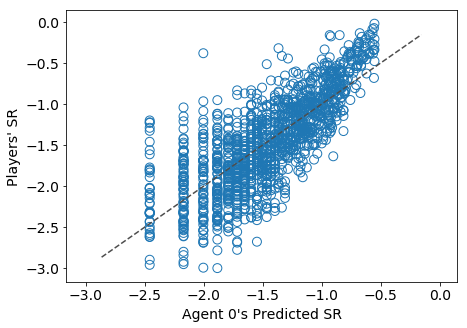
\includegraphics[width=0.3\textwidth]{masters-thesis-master/masters-thesis/contents/a_appendix/assumption_validation/pred_obs/a0.png}
    \label{fig:assamp_val:pred_obs_a0}
    }
    \subfloat[Agent 1]{
    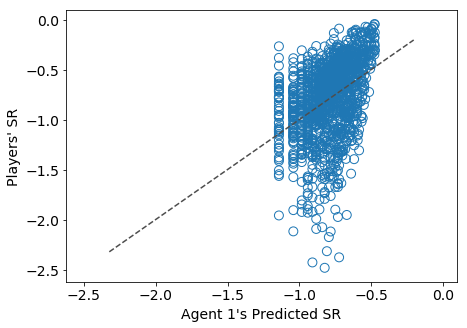
\includegraphics[width=0.3\textwidth]{masters-thesis-master/masters-thesis/contents/a_appendix/assumption_validation/pred_obs/a1.png}
    \label{fig:assamp_val:pred_obs_a1}
    }
  \subfloat[Agent 2]{
    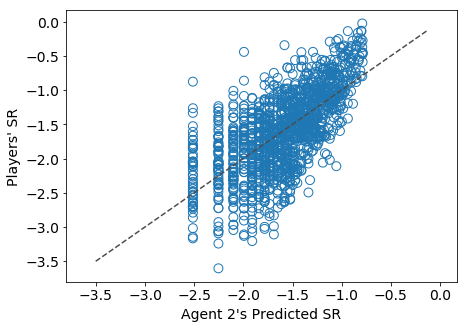
\includegraphics[width=0.3\textwidth]{masters-thesis-master/masters-thesis/contents/a_appendix/assumption_validation/pred_obs/a2.png}
    \label{fig:assamp_val:pred_obs_a2}
    }
    
  \subfloat[Agent 3]{
    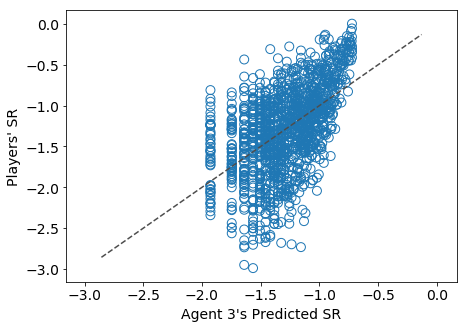
\includegraphics[width=0.3\textwidth]{masters-thesis-master/masters-thesis/contents/a_appendix/assumption_validation/pred_obs/a3.png}
    \label{fig:assamp_val:pred_obs_a3}
    }
    \subfloat[Agent 4]{
    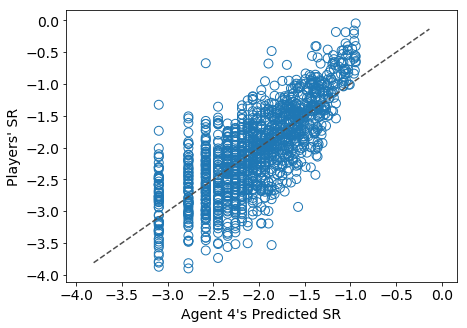
\includegraphics[width=0.3\textwidth]{masters-thesis-master/masters-thesis/contents/a_appendix/assumption_validation/pred_obs/a4.png}
    \label{fig:assamp_val:pred_obs_a4}
    }
  \subfloat[Agent 5]{
    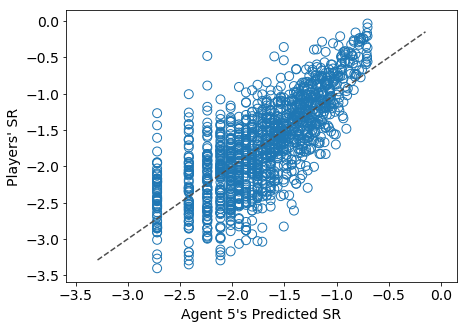
\includegraphics[width=0.3\textwidth]{masters-thesis-master/masters-thesis/contents/a_appendix/assumption_validation/pred_obs/a5.png}
    \label{fig:assamp_val:pred_obs_a5}
    }
    \caption{Players' SR against predicted SR}
    \label{fig:assamp_val:pred_obs}
\end{figure}

\begin{figure}[H]
  \centering
  \subfloat[Agent 0]{
    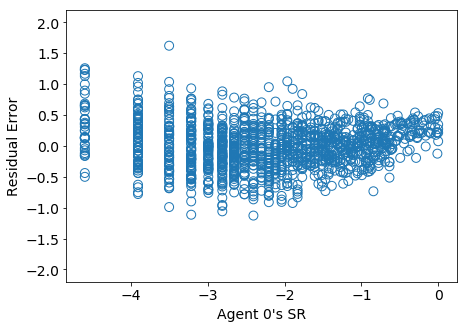
\includegraphics[width=0.3\textwidth]{masters-thesis-master/masters-thesis/contents/a_appendix/assumption_validation/res_sr/a0.png}
    \label{fig:assamp_val:res_sr_a0}
    }
    \subfloat[Agent 1]{
    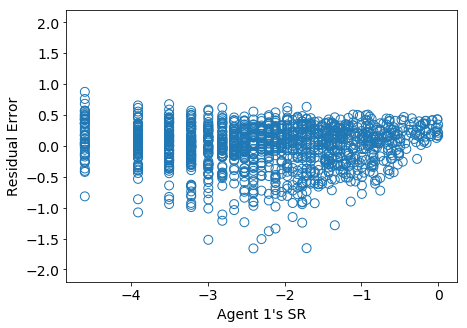
\includegraphics[width=0.3\textwidth]{masters-thesis-master/masters-thesis/contents/a_appendix/assumption_validation/res_sr/a1.png}
    \label{fig:assamp_val:res_sr_a1}
    }
  \subfloat[Agent 2]{
    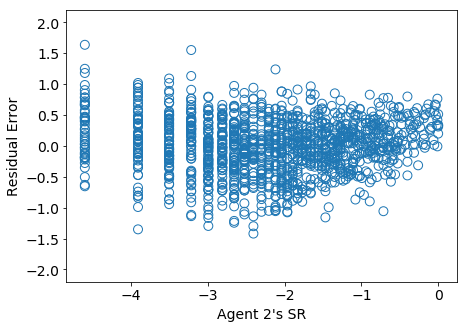
\includegraphics[width=0.3\textwidth]{masters-thesis-master/masters-thesis/contents/a_appendix/assumption_validation/res_sr/a2.png}
    \label{fig:assamp_val:res_sr_a2}
    }
    
  \subfloat[Agent 3]{
    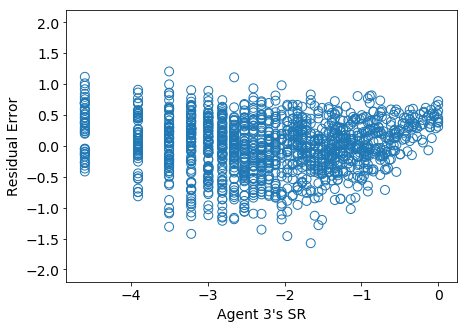
\includegraphics[width=0.3\textwidth]{masters-thesis-master/masters-thesis/contents/a_appendix/assumption_validation/res_sr/a3.png}
    \label{fig:assamp_val:res_sr_a3}
    }
    \subfloat[Agent 4]{
    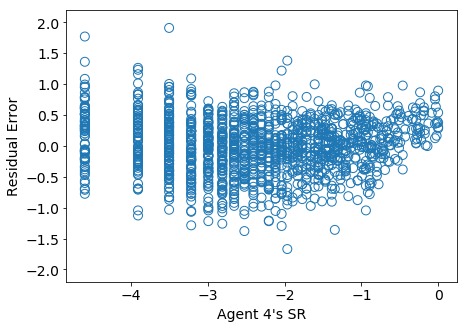
\includegraphics[width=0.3\textwidth]{masters-thesis-master/masters-thesis/contents/a_appendix/assumption_validation/res_sr/a4.png}
    \label{fig:assamp_val:res_sr_a4}
    }
  \subfloat[Agent 5]{
    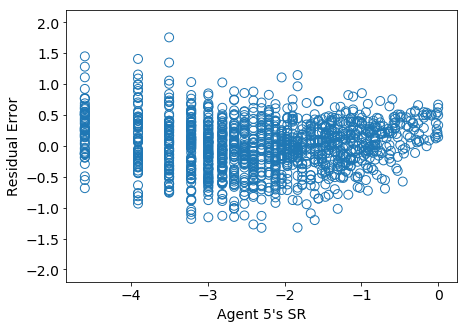
\includegraphics[width=0.3\textwidth]{masters-thesis-master/masters-thesis/contents/a_appendix/assumption_validation/res_sr/a5.png}
    \label{fig:assamp_val:res_sr_a5}
    }
    \caption{Agent's SR against residuals}
    \label{fig:assamp_val:res_sr}
\end{figure}


\begin{figure}[h]
  \centering
  \subfloat[Agent 0]{
    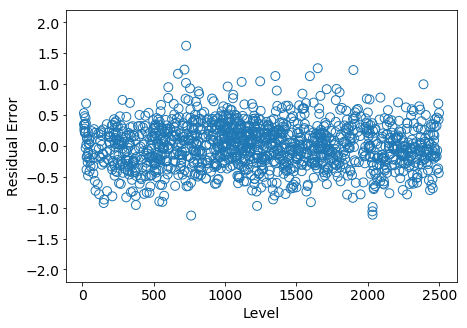
\includegraphics[width=0.31\textwidth]{masters-thesis-master/masters-thesis/contents/a_appendix/assumption_validation/res_levels/a0.png}
    \label{fig:assamp_val:res_levels_a0}
    }
    \subfloat[Agent 1]{
    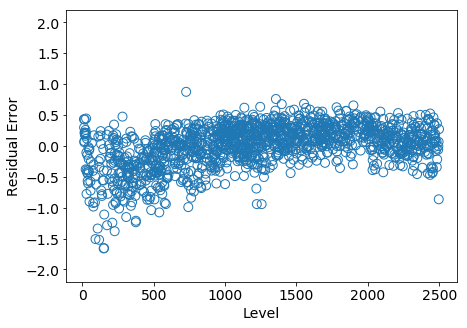
\includegraphics[width=0.31\textwidth]{masters-thesis-master/masters-thesis/contents/a_appendix/assumption_validation/res_levels/a1.png}
    \label{fig:assamp_val:res_levels_a1}
    }
  \subfloat[Agent 2]{
    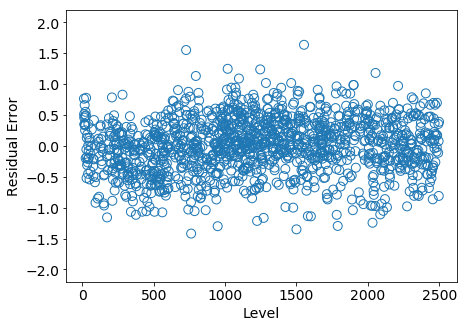
\includegraphics[width=0.31\textwidth]{masters-thesis-master/masters-thesis/contents/a_appendix/assumption_validation/res_levels/a2.png}
    \label{fig:assamp_val:res_levels_a2}
    }
    
  \subfloat[Agent 3]{
    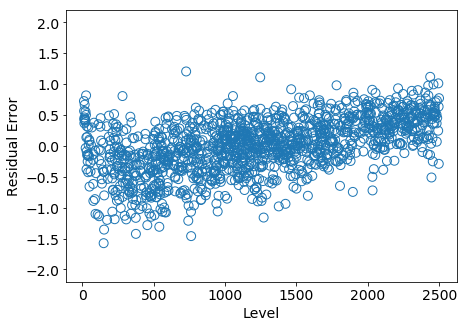
\includegraphics[width=0.31\textwidth]{masters-thesis-master/masters-thesis/contents/a_appendix/assumption_validation/res_levels/a3.png}
    \label{fig:assamp_val:res_levels_a3}
    }
    \subfloat[Agent 4]{
    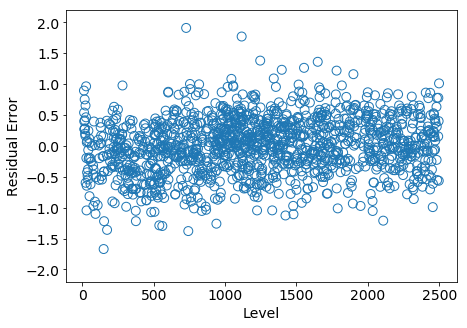
\includegraphics[width=0.31\textwidth]{masters-thesis-master/masters-thesis/contents/a_appendix/assumption_validation/res_levels/a4.png}
    \label{fig:assamp_val:res_levels_a4}
    }
  \subfloat[Agent 5]{
    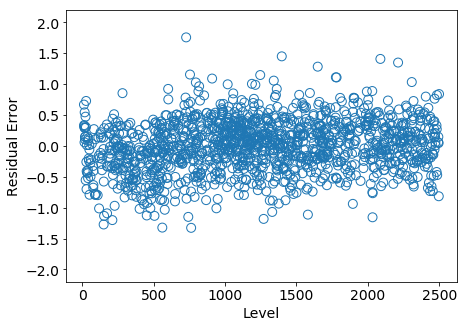
\includegraphics[width=0.31\textwidth]{masters-thesis-master/masters-thesis/contents/a_appendix/assumption_validation/res_levels/a5.png}
    \label{fig:assamp_val:res_levels_a5}
    }
    \caption{Levels against residuals}
    \label{fig:assamp_val:res_levels}
\end{figure}

\begin{figure}[H]
  \centering
  \subfloat[Agent 0]{
    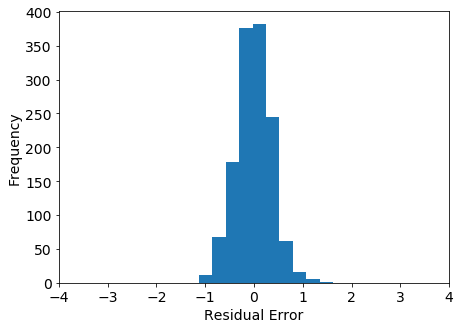
\includegraphics[width=0.31\textwidth]{masters-thesis-master/masters-thesis/contents/a_appendix/assumption_validation/freq/a0.png}
    \label{fig:assamp_val:freq_a0}
    }
    \subfloat[Agent 1]{
    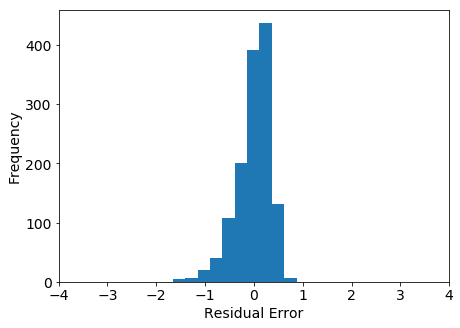
\includegraphics[width=0.31\textwidth]{masters-thesis-master/masters-thesis/contents/a_appendix/assumption_validation/freq/a1.png}
    \label{fig:assamp_val:freq_a1}
    }
  \subfloat[Agent 2]{
    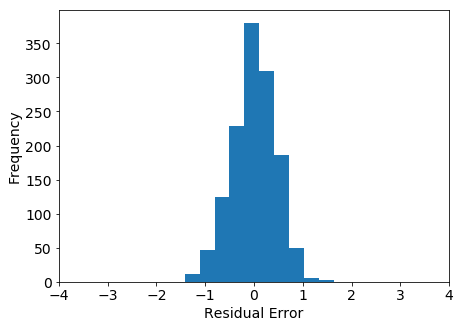
\includegraphics[width=0.31\textwidth]{masters-thesis-master/masters-thesis/contents/a_appendix/assumption_validation/freq/a2.png}
    \label{fig:assamp_val:freq_a2}
    }
    
  \subfloat[Agent 3]{
    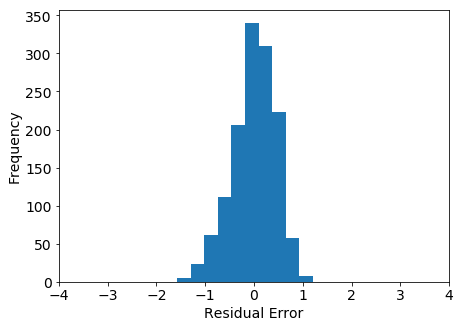
\includegraphics[width=0.31\textwidth]{masters-thesis-master/masters-thesis/contents/a_appendix/assumption_validation/freq/a3.png}
    \label{fig:assamp_val:freq_a3}
    }
    \subfloat[Agent 4]{
    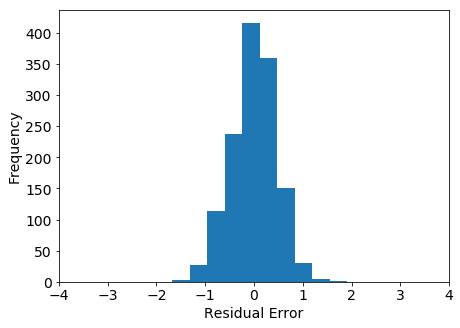
\includegraphics[width=0.31\textwidth]{masters-thesis-master/masters-thesis/contents/a_appendix/assumption_validation/freq/a4.png}
    \label{fig:assamp_val:freq_a4}
    }
  \subfloat[Agent 5]{
    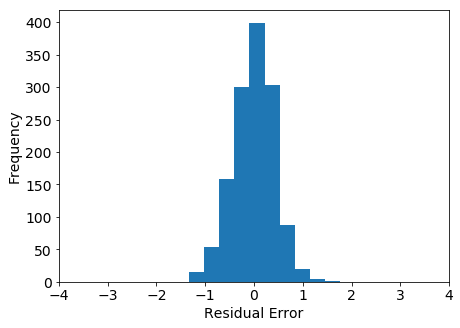
\includegraphics[width=0.31\textwidth]{masters-thesis-master/masters-thesis/contents/a_appendix/assumption_validation/freq/a5.png}
    \label{fig:assamp_val:freq_a5}
    }
    \caption{Residual frequency}
    \label{fig:assamp_val:freq}
\end{figure}

\begin{figure}[H]
  \centering
  \subfloat[Agent 0]{
    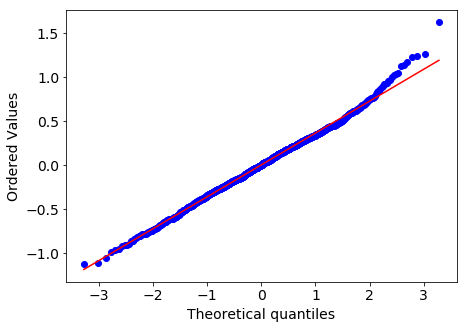
\includegraphics[width=0.31\textwidth]{masters-thesis-master/masters-thesis/contents/a_appendix/assumption_validation/qq/a0.png}
    \label{fig:assamp_val:qq_a0}
    }
    \subfloat[Agent 1]{
    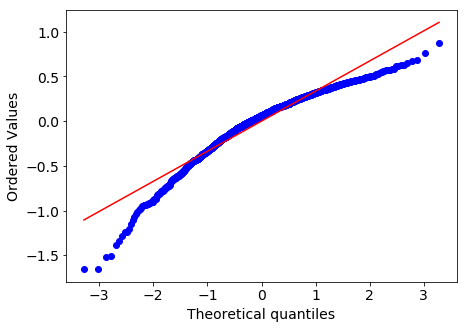
\includegraphics[width=0.31\textwidth]{masters-thesis-master/masters-thesis/contents/a_appendix/assumption_validation/qq/a1.png}
    \label{fig:assamp_val:qq_a1}
    }
  \subfloat[Agent 2]{
    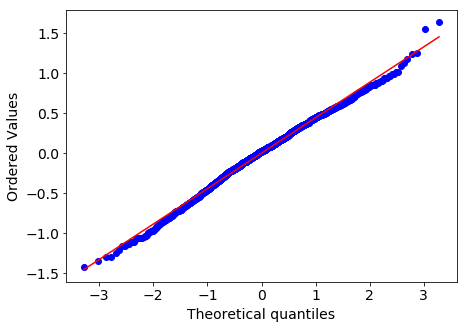
\includegraphics[width=0.31\textwidth]{masters-thesis-master/masters-thesis/contents/a_appendix/assumption_validation/qq/a2.png}
    \label{fig:assamp_val:qq_a2}
    }
    
  \subfloat[Agent 3]{
    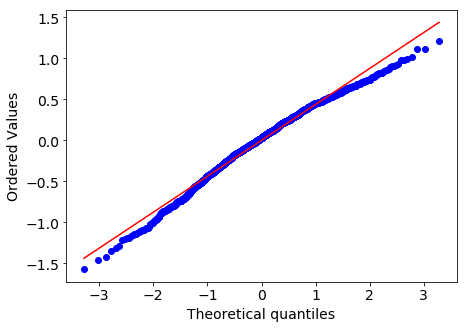
\includegraphics[width=0.31\textwidth]{masters-thesis-master/masters-thesis/contents/a_appendix/assumption_validation/qq/a3.png}
    \label{fig:assamp_val:qq_a3}
    }
    \subfloat[Agent 4]{
    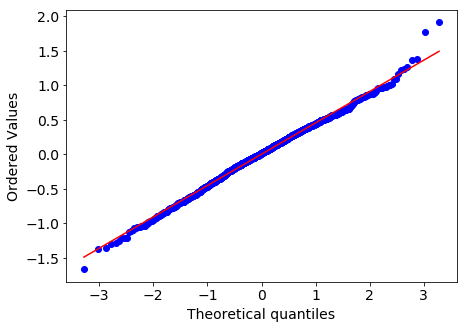
\includegraphics[width=0.31\textwidth]{masters-thesis-master/masters-thesis/contents/a_appendix/assumption_validation/qq/a4.png}
    \label{fig:assamp_val:qq_a4}
    }
  \subfloat[Agent 5]{
    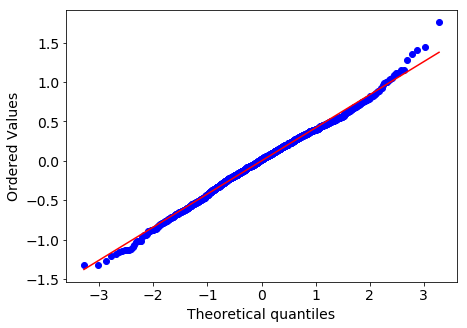
\includegraphics[width=0.31\textwidth]{masters-thesis-master/masters-thesis/contents/a_appendix/assumption_validation/qq/a5.png}
    \label{fig:assamp_val:qq_a5}
    }
    \caption{Normal probability plots of residuals}
    \label{fig:assamp_val:qq}
\end{figure}

\begin{figure}[H]
  \centering
  \subfloat[Players' vs predicted SR]{
  \centering
    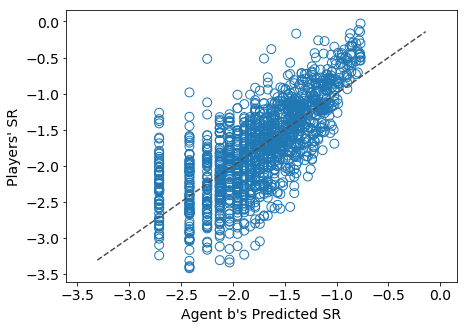
\includegraphics[width=0.31\textwidth]{masters-thesis-master/masters-thesis/contents/a_appendix/assumption_validation/baseline/b0.png}
    \label{fig:assamp_val:baseline_b0}
    }
    \subfloat[Baseline's SR vs residuals]{
    \centering
    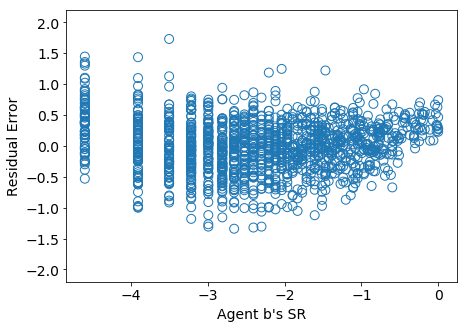
\includegraphics[width=0.31\textwidth]{masters-thesis-master/masters-thesis/contents/a_appendix/assumption_validation/baseline/b1.png}
    \label{fig:assamp_val:baseline_b1}
    }
  \subfloat[Levels vs residuals]{
  \centering
    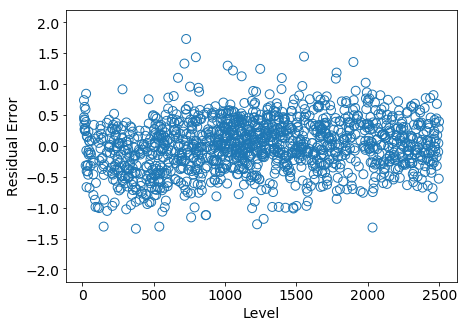
\includegraphics[width=0.31\textwidth]{masters-thesis-master/masters-thesis/contents/a_appendix/assumption_validation/baseline/b2.png}
    \label{fig:assamp_val:baseline_b2}
    }
    
  \subfloat[Residual frequency]{
  \centering
    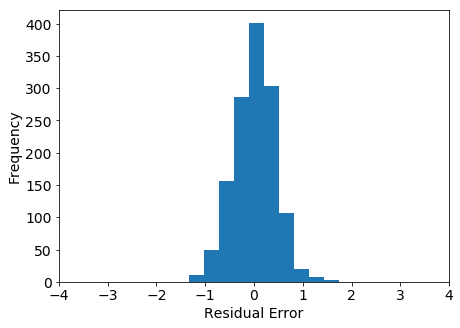
\includegraphics[width=0.31\textwidth]{masters-thesis-master/masters-thesis/contents/a_appendix/assumption_validation/baseline/b3.png}
    \label{fig:assamp_val:baseline_b3}
    }
    \subfloat[Residual normal prob. plot]{

    \includegraphics[width=0.315\textwidth]{masters-thesis-master/masters-thesis/contents/a_appendix/assumption_validation/baseline/b4.png}
    \centering
    \label{fig:assamp_val:baseline_b4}
    }
    \caption{Assumptions validation for the baseline}
    \label{fig:assamp_val:baseline}
\end{figure}
\newpage
\subsection{Agents' and Baseline's Predictions in the Player Clusters}\label{predictions_comparison}
\begin{figure}[H]
  \centering
  \subfloat[Agent 0's predictions]{
    \includegraphics[width=0.4\textwidth]{masters-thesis-master/masters-thesis/contents/a_appendix/agents_baseline_player_clusters/a0.png}
    \label{fig:predictions_comparison:a0}
    }
    \subfloat[Baseline's predictions for cluster 0]{
    \includegraphics[width=0.4\textwidth]{masters-thesis-master/masters-thesis/contents/a_appendix/agents_baseline_player_clusters/b0.png}
    \label{fig:predictions_comparison:bo}
    }
    
  \subfloat[Agent 1's predictions]{
    \includegraphics[width=0.4\textwidth]{masters-thesis-master/masters-thesis/contents/a_appendix/agents_baseline_player_clusters/a1.png}
    \label{fig:predictions_comparison:a1}
    }
  \subfloat[Baseline's predictions for cluster 1]{
    \includegraphics[width=0.4\textwidth]{masters-thesis-master/masters-thesis/contents/a_appendix/agents_baseline_player_clusters/b1.png}
    \label{fig:predictions_comparison:b1}
    }
      
  \subfloat[Agent 2's predictions]{
    \includegraphics[width=0.4\textwidth]{masters-thesis-master/masters-thesis/contents/a_appendix/agents_baseline_player_clusters/a2.png}
    \label{fig:predictions_comparison:a2}
    }
  \subfloat[Baseline's predictions for cluster 2]{
    \includegraphics[width=0.4\textwidth]{masters-thesis-master/masters-thesis/contents/a_appendix/agents_baseline_player_clusters/b2.png}
    \label{fig:predictions_comparison:b2}
    }
    \caption{Agents' vs baseline's predictions on each player cluster (1/2)}
    \label{fig:predictions_comparison_1}
\end{figure}

\begin{figure}[H]
  \centering
  \subfloat[Agent 3's predictions]{
    \includegraphics[width=0.4\textwidth]{masters-thesis-master/masters-thesis/contents/a_appendix/agents_baseline_player_clusters/a3.png}
    \label{fig:predictions_comparison:a3}
    }
  \subfloat[Baseline's predictions for cluster 3]{
    \includegraphics[width=0.4\textwidth]{masters-thesis-master/masters-thesis/contents/a_appendix/agents_baseline_player_clusters/b3.png}
    \label{fig:predictions_comparison:b3}
    }
    
  \subfloat[Agent 4's predictions]{
    \includegraphics[width=0.4\textwidth]{masters-thesis-master/masters-thesis/contents/a_appendix/agents_baseline_player_clusters/a4.png}
    \label{fig:predictions_comparison:a4}
    }
  \subfloat[Baseline's predictions for cluster 4]{
    \includegraphics[width=0.4\textwidth]{masters-thesis-master/masters-thesis/contents/a_appendix/agents_baseline_player_clusters/b4.png}
    \label{fig:predictions_comparison:b4}
    }
    
  \subfloat[Agent 5's predictions]{
    \includegraphics[width=0.4\textwidth]{masters-thesis-master/masters-thesis/contents/a_appendix/agents_baseline_player_clusters/a5.png}
    \label{fig:predictions_comparison:a5}
    }
  \subfloat[Baseline's predictions for cluster 5]{
    \includegraphics[width=0.4\textwidth]{masters-thesis-master/masters-thesis/contents/a_appendix/agents_baseline_player_clusters/b5.png}
    \label{fig:predictions_comparison:b5}
    }
    \caption{Agents' vs baseline's predictions on each player cluster (2/2)}
    \label{fig:predictions_comparison_2}
\end{figure}

\section{Supplement Plots for the Clustering Simulated Strategies Approach}

\subsection{Assumptions Validation on Training Levels Plots}\label{assamp_val_sim_strategies}

\begin{figure}[h!]
  \centering
  \subfloat[Agents' vs predicted SR]{
  \centering
    \includegraphics[width=0.31\textwidth]{masters-thesis-master/masters-thesis/contents/a_appendix/assumption_validation/sim_strategies_train_agents/a0.png}
    \label{fig:assamp_val:train_agents_a0}
    }
    \subfloat[Avg agents' SR vs residuals]{
    \centering
    \includegraphics[width=0.31\textwidth]{masters-thesis-master/masters-thesis/contents/a_appendix/assumption_validation/sim_strategies_train_agents/a1.png}
    \label{fig:assamp_val:train_agentse_a1}
    }
  \subfloat[Levels vs residuals]{
  \centering
    \includegraphics[width=0.31\textwidth]{masters-thesis-master/masters-thesis/contents/a_appendix/assumption_validation/sim_strategies_train_agents/a2.png}
    \label{fig:assamp_val:train_agents_a2}
    }
    
  \subfloat[Residual frequency]{
  \centering
    \includegraphics[width=0.31\textwidth]{masters-thesis-master/masters-thesis/contents/a_appendix/assumption_validation/sim_strategies_train_agents/a3.png}
    \label{fig:assamp_val:train_agents_a3}
    }
    \subfloat[Residual normal prob. plot]{
    \includegraphics[width=0.31\textwidth]{masters-thesis-master/masters-thesis/contents/a_appendix/assumption_validation/sim_strategies_train_agents/a4.png}
    \centering
    \label{fig:assamp_val:train_agents_a4}
    }
    \caption{Assumptions validation for the agents' linear model}
    \label{fig:assamp_val:train_agents}
\end{figure}

\begin{figure}[h]
  \centering
  \subfloat[Baseline's vs predicted SR]{
  \centering
    \includegraphics[width=0.31\textwidth]{masters-thesis-master/masters-thesis/contents/a_appendix/assumption_validation/sim_strategies_train_base/b0.png}
    \label{fig:assamp_val:train_base_b0}
    }
    \subfloat[Baseline's SR vs residuals]{
    \centering
    \includegraphics[width=0.31\textwidth]{masters-thesis-master/masters-thesis/contents/a_appendix/assumption_validation/sim_strategies_train_base/b1.png}
    \label{fig:assamp_val:train_base_b1}
    }
  \subfloat[Levels vs residuals]{
  \centering
    \includegraphics[width=0.31\textwidth]{masters-thesis-master/masters-thesis/contents/a_appendix/assumption_validation/sim_strategies_train_base/b2.png}
    \label{fig:assamp_val:train_base_b2}
    }
    
  \subfloat[Residual frequency]{
  \centering
    \includegraphics[width=0.31\textwidth]{masters-thesis-master/masters-thesis/contents/a_appendix/assumption_validation/sim_strategies_train_base/b3.png}
    \label{fig:assamp_val:train_base_b3}
    }
    \subfloat[Residuals normal prob. plot]{

    \includegraphics[width=0.31\textwidth]{masters-thesis-master/masters-thesis/contents/a_appendix/assumption_validation/sim_strategies_train_base/b4.png}
    \centering
    \label{fig:assamp_val:train_base_b4}
    }
    \caption{Assumptions validation for the baseline's linear model}
    \label{fig:assamp_val:train_base}
\end{figure}
